\chapter{Cloud Domain Infrastructure/Architecture}

\section{Cloud system overview}
'Benchmarking Cloud Serving Systems with YCSB' : 'Classification of Systems and Tradeoffs'
Read performance versus write performance, Latency versus durability, Synchronous versus asynchronous replication, Data partitioning


'Toward a Unified Ontologyof Cloud Computing' - Kan bruges til indledning omkring cloud computing

\section{Consistency}
Client-centric Benchmarking of Eventual Consistency for Cloud Storage Systems: "client-centric consistency, which captures what client applications observe directly, or system-centric consistency, which captures the convergence of the storage system’s replication protocol"

'Toward a Principled Framework for Benchmarking Consistency'
He total order extends the “happens before” partial order (i.e., if operation A ended before op- eration B began during the execution, then A precedes B in the total order);

\section{Availability}
'Benchmarking Cloud Serving Systems with YCSB'

"Replication is used to improve system availability (by directing traffic to a replica after a failure), avoid data loss (by recovering lost data from a replica), and improve performance (by spreading load across multiple replicas and by making low-latency access available to users around the world)."

\section{Cluster management}

\url{https://www.nomadproject.io/intro/vs/ecs.html}

\subparagraph{Kubernetes}

\url{https://kubernetes.io/docs/whatisk8s/}

\section{Containerization}



\subsection{RKT}

\url{https://aptira.com/coreos-rkt/}

\subsection{Measurement points}
How does the amount of data stored affect the performance?
How is consistency managed?

\subsection*{Noter}
The thought of microservies is not new. But the accessibility and knowledge sharing is.

\url{https://en.wikipedia.org/wiki/Cloud_computing#Infrastructure_as_a_service_.28IaaS.29}

Infrastructure as a service  (IaaS)

Platform as a service (Paas) \url{https://en.wikipedia.org/wiki/Platform_as_a_service}

Software as a service (SaaS)

Mobile backend as a service MBaaS \url{https://en.wikipedia.org/wiki/Mobile_backend_as_a_service}

DevOps

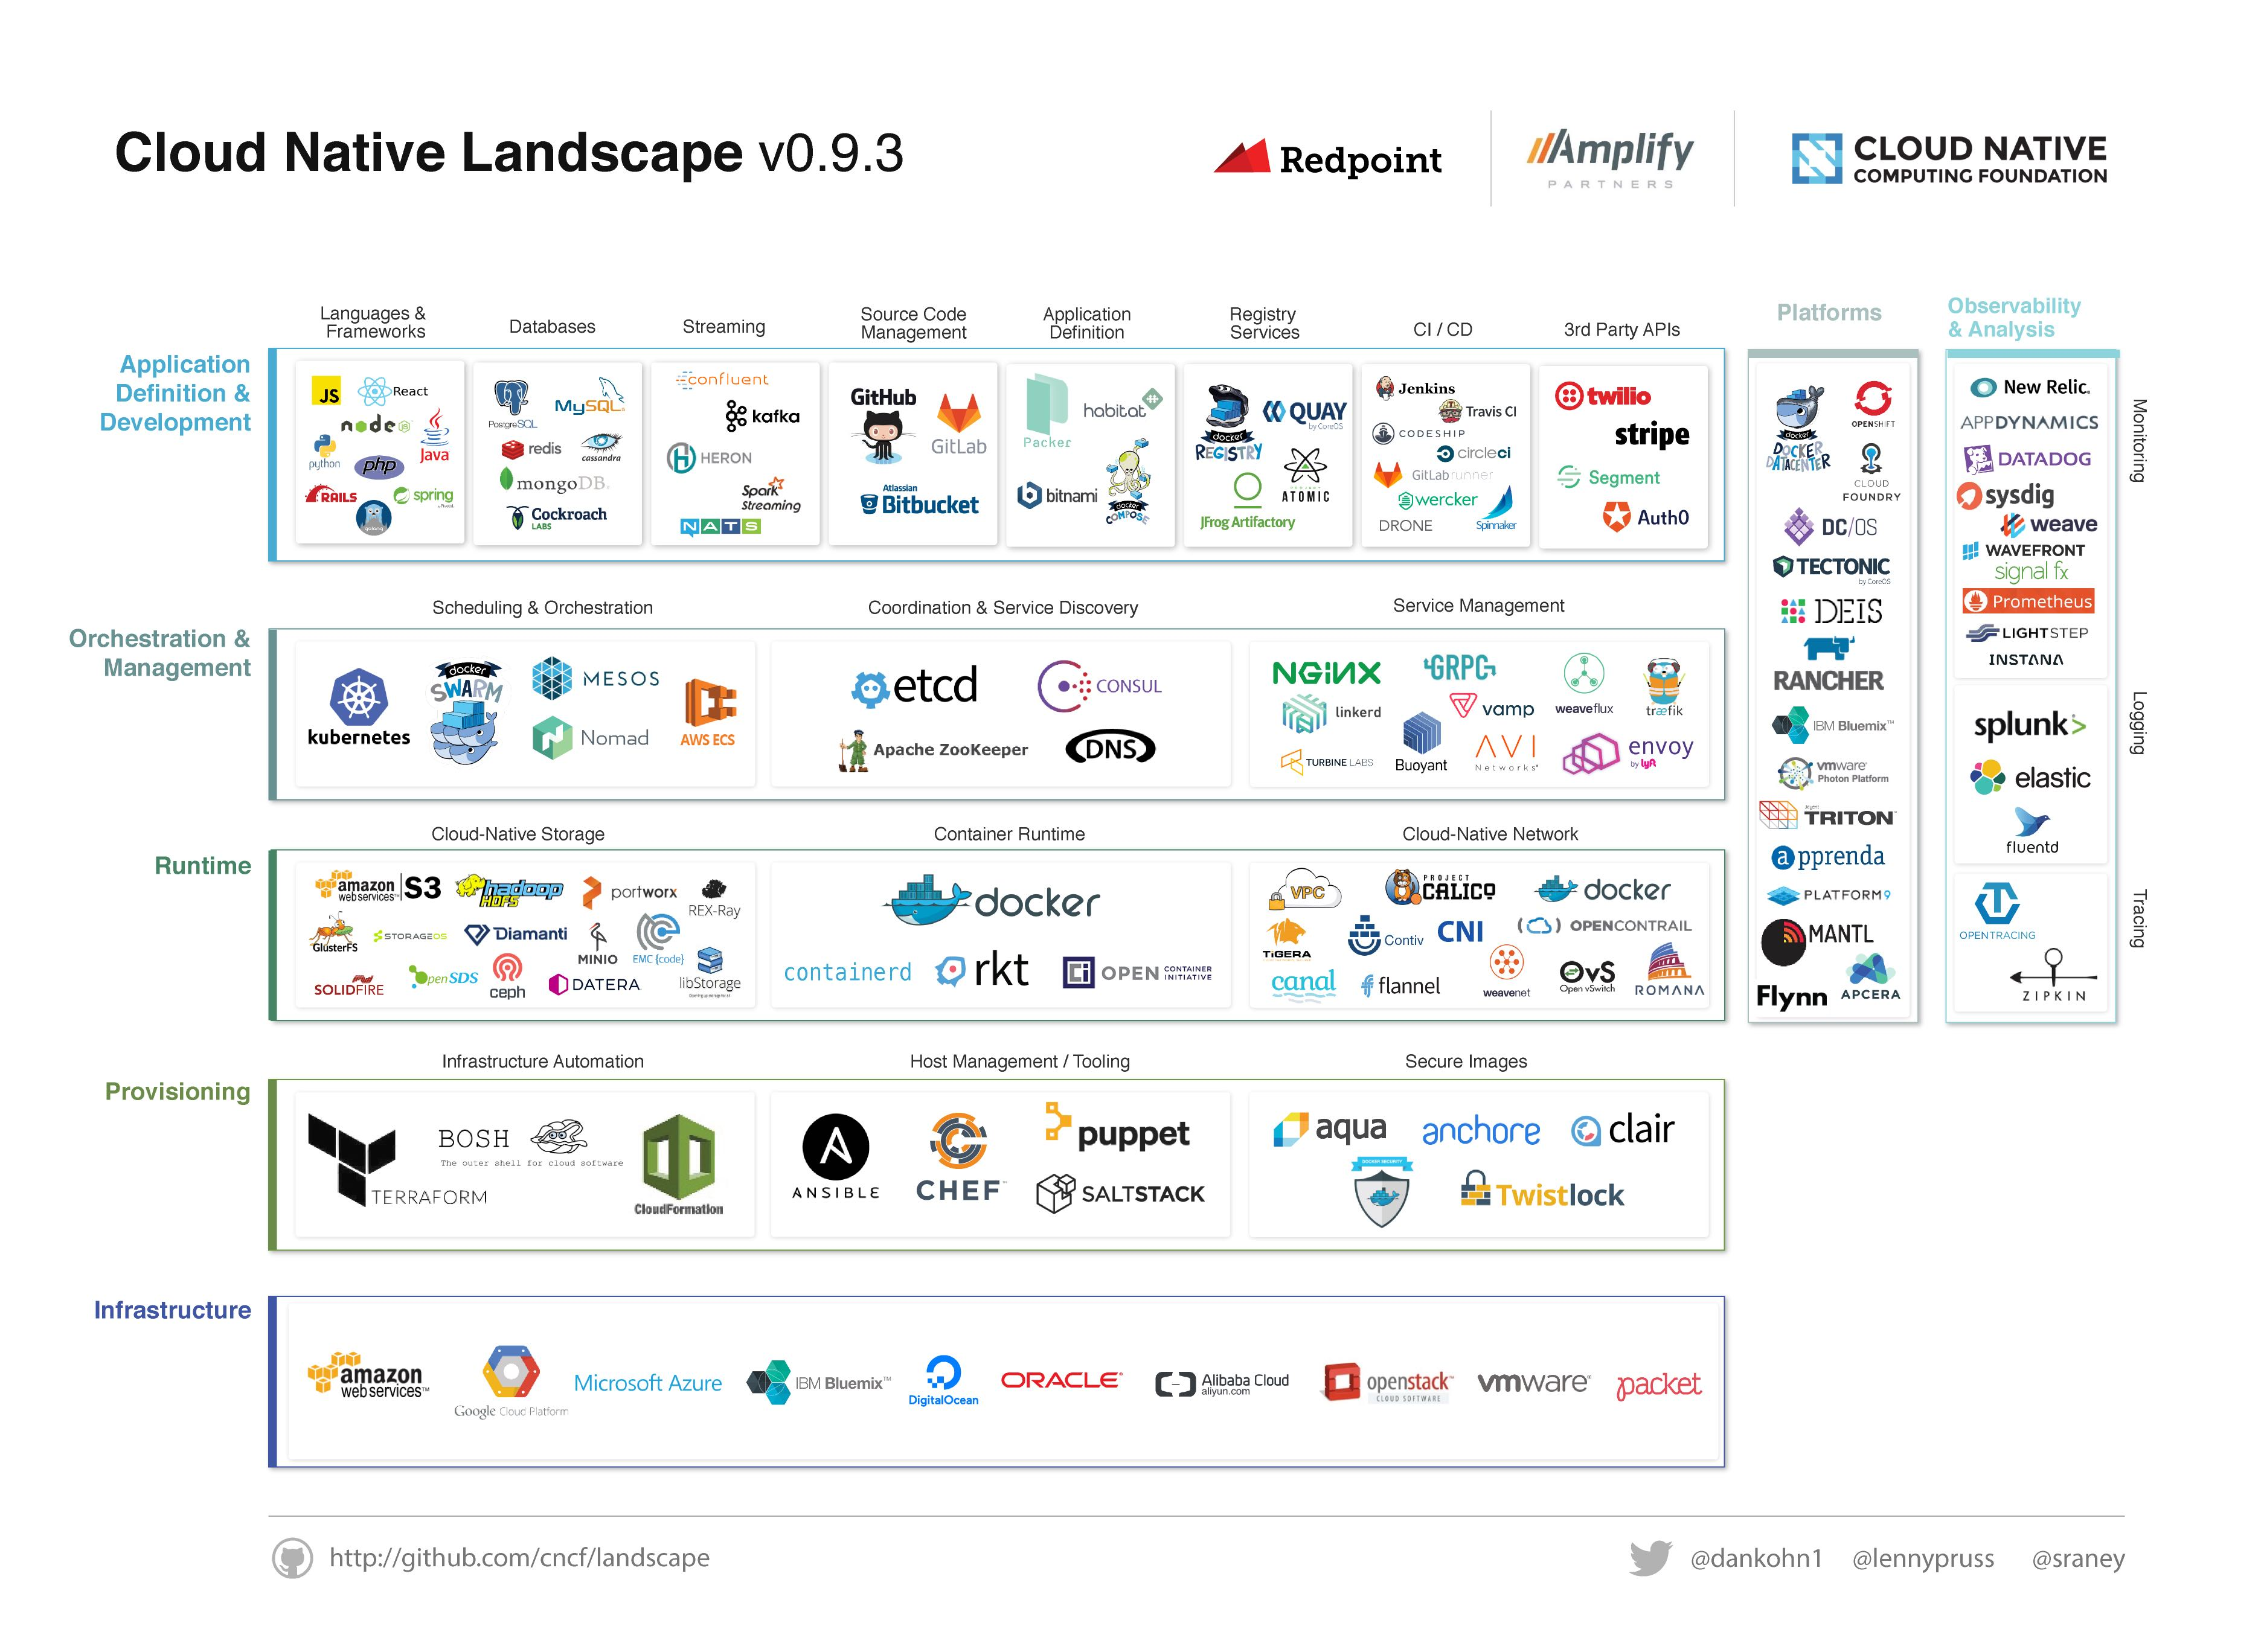
\includegraphics[scale=0.12]{cloudnativelandscape}

\subsection*{Notes}
Service Oriented Architectures \url{https://en.wikipedia.org/wiki/Service-oriented_architecture}


\subsection{Microservices: Theory and Application}
\url{https://www.youtube.com/watch?v=bHqRxMwfrng}

Monolith:
Typically kind of bad, as they grow and get more and more unmaintainable the cost of maintenance outpases the outweighs the benefits. Implementing a new feature takes a long time.

Mircroservices:
Domain driven design, understand what you are building. Break apart your business functions around bounded context, a bounded context per service.

Principals

\begin{itemize}
\item Encapsulation
\item Automation
\item Domain centric
\item Decentralized
\item Independent
\item Fail-safe
\item Observable
\end{itemize}

Scalability 

Shift to maintainability. Writing fine grained very focused micro services. It is modular, easier readable, understandable.

'Sea change' - Time is ripe. Automation, containers, Dev-Ops, higher level abstraction.

Team structure should usually be a holistic end to end team QA, product management, developers, release engineers, working together front to end. They own the product, service and so on. Ties the team together.

Partitioning strategy Verb or use-case, noun or resource, grouping things that change together. Single responsibility principle.

Benefits. Faster deployment. Easier to test. Scalability.

Challenges.
More complexity. System testing. Distributed transactions, (eventual consistency). Management of system.
Organization and culture, maturity.

Netflix
\url{https://www.youtube.com/watch?v=57UK46qfBLY}
Microservice failure
\begin{itemize}
\item Hystrix
\item Chaos monkey
\item Fault-injection test framework
\end{itemize}
